% !TEX root = ../../../main.tex

\toggletrue{image}
\toggletrue{imagehover}
\chapterimage{wardrobe}
\chapterimagetitle{\uppercase{Wardrobe}}
\chapterimageurl{https://xkcd.com/2218/}
\chapterimagehover{If you'd just agree to hold your meetings in here, you'd have PLENTY of time to figure things out before the deadline.}

\chapter{Schlüsselverteilung mit einer Truhe}
\label{chapter-schluesselverteilung-truhe}

\vspace{-0.5cm}

Mit einer abschliessbaren Truhe, zwei Vorhängeschlössern und einem Kurier verteilen wir einen gemeinsamen Schlüssel. Das Lernziel lautet:

\newcommand{\schluesselverteilungTruheLernziele}{
\protect\begin{todolist}
\item Sie erklären und wenden das Protokoll \texttt{SCHLÜSSELVERTEILUNG TRUHE} an.
\end{todolist}
}

\lernziel{\autoref{chapter-schluesselverteilung-truhe}, \nameref{chapter-schluesselverteilung-truhe}}{\protect\schluesselverteilungTruheLernziele}

\vspace{-0.25cm}

\schluesselverteilungTruheLernziele

\section{Protokoll \texttt{SCHLÜSSELVERTEILUNG TRUHE}}

Das Prinzip ist überraschend einfach und in \autoref{figure-schluesselverteilung-truhe} dargestellt. Die Truhe verschicken wir mit einem Kurier. Alice und Bob müssen sich nicht treffen.

\begin{figure}[htb]
	\centering
	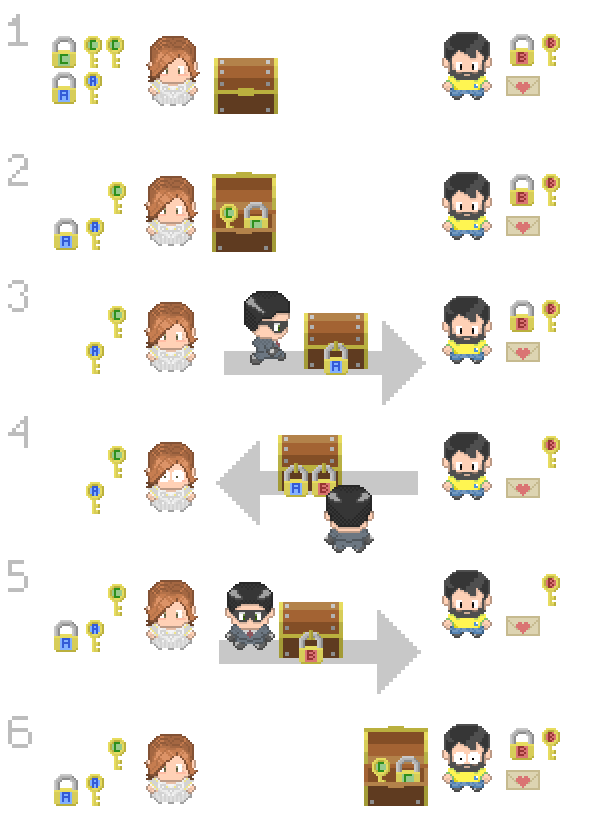
\includegraphics[scale=0.36]{schluesselverteilung_truhe_1}
	\caption{Eve ist eine \textbf{passive} Angreiferin und setzt keine Gewalt ein!}
	\label{figure-schluesselverteilung-truhe}
\end{figure}

\vspace{-0.25cm}

\begin{important}
	Die Truhe wird \textbf{nie} ohne Vorhängeschloss verschickt! Am Ende besitzen beide den \textbf{grünen Schlüssel}. Dies ist der \textbf{gemeinsame} Schlüssel.
\end{important}

\section{Verschlüsselte Kommunikation}

Alice und Bob können nun wie gewohnt sicher kommunizieren. Sie verwenden die Truhe und das grüne Vorhängeschloss (Buchstabe C). Beide besitzen den passenden, grünen Schlüssel (Buchstabe C). Sie verwenden den Schlüssel, um die Truhe zu verschliessen und wieder zu öffnen. Die Kommunikation mit dem grünen Vorhängeschloss und den grünen Schlüsseln entspricht somit einem \textbf{symmetrischen} Kryptosystem. \autoref{figure-gruener-schluessel} zeigt die Idee.

\begin{figure}[htb]
	\centering
	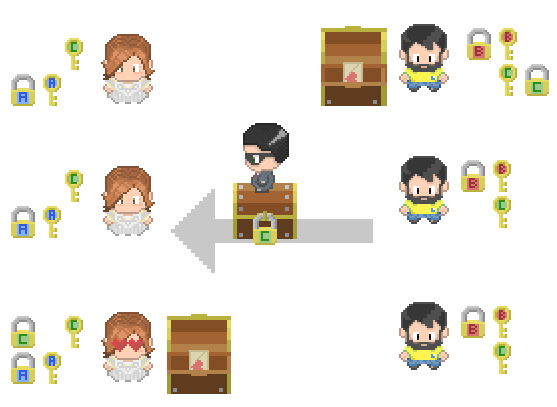
\includegraphics[scale=0.55]{schluesselverteilung_truhe_2}
	\caption{Eve besitzt den grünen Schlüssel nicht und kann die Nachricht nicht lesen.}
	\label{figure-gruener-schluessel}
\end{figure}

\section{Aufgaben}

\begin{enumerate}
\item Darf auch Bob den Schlüssel bei der \say{Schlüsselverteilung mit einer Truhe} bestimmen und an Alice verteilen? Begründen Sie Ihre Antwort.

\fillwithgrid{1in}

\item Alice macht folgenden Vorschlag: Das Prinzip der \say{Schlüsselverteilung mit einer Truhe} wird nicht zum Verteilen des Schlüssels benutzt, sondern zur Übermittlung einer Nachricht.
\begin{enumerate}
\item Ist die Idee von Alice möglich? Begründen Sie Ihre Antwort.

\fillwithgrid{2in}

\item Überlegen Sie sich mindestens einen Grund, warum wir nicht direkt die Nachricht übermitteln, sondern einen gemeinsamen Schlüssel.

\fillwithgrid{2in}

\end{enumerate}

\item Alice möchte nun auch noch mit Carol verschlüsselt kommunizieren. Die verschlüsselte Kommunikation zu Bob soll weiterhin möglich sein. Wie muss Alice nun bei der Schlüsselverteilung vorgehen?

\fillwithgrid{3in}

\item Es möchten nun $n$ Personen miteinander verschlüsselt kommunizieren.

\begin{enumerate}
\item Wie viele Schlüssel benötigt eine Person? Es soll zu jeder anderen Person eine verschlüsselte $1:1$-Kommunikation möglich sein. Begründen Sie Ihre Berechnung.

\fillwithgrid{1in}

\item Wie viele Schlüssel gibt es insgesamt? Notieren Sie eine Formel mit einer Begründung.

\fillwithgrid{1in}

\end{enumerate}

\end{enumerate}
